\documentclass[11pt, a4paper]{article}

\usepackage[margin=1in]{geometry} % manage page dimentions
\usepackage[utf8]{inputenc} % utf-8 encoding
\usepackage[italian]{babel} % italian default text
\usepackage[hidelinks]{hyperref} % link references
\usepackage{bookmark} % 
\usepackage{import} % import other .tex files
\usepackage{amsmath} % math commands
\usepackage{amssymb} % math symbols
\usepackage{amsthm} % math environments
\usepackage{amsmath} % equation align
\usepackage{siunitx} % SI unit
\usepackage{booktabs} % tabular enhance
\usepackage{multirow} % dinamic tabular cell dimentions
\usepackage{longtable} % multi-page table
\usepackage[labelfont=bf, skip=.5em, font=small]{caption} % beautiful caption
\usepackage{subcaption} % subfigure
\usepackage{graphicx} % import graphics
\usepackage{fancyhdr} % custom page header and footer

\graphicspath{{../assets/}} % base graphics path

\setlength{\parskip}{1em} % distance between paragraphs
\setlength{\parindent}{0em} % indentation at beginning of paragraph

\numberwithin{equation}{section} % equation tag relative to section

\title{Esperienza 3}
\author{Matteo Romano, Vittorio Strano}
\date{09/12/2021}

\begin{document}

\maketitle

\tableofcontents

\section{Obiettivo dell'esperienza}

Lo scopo dell'esperienza è quello di calcolare il valore della resistenza e della capacità di un circuito RC. Per farlo si analizza la differenza di potenziale ai capi di R (\autoref{fig:circuito R}) e/o ai capi di C (\autoref{fig:circuito C}) quando si sottopone il circuito ad una tensione variabile.

\begin{figure}[ht!]
    \centering
    \begin{subfigure}[c]{.3\textwidth}
        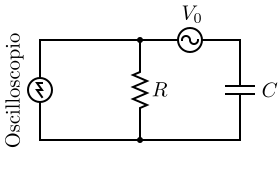
\includegraphics[width=\textwidth]{circuito_osc_R.pdf}
        \caption{Misure ai capi di R}
        \label{fig:circuito R}
    \end{subfigure}
    \hspace{1in}
    \begin{subfigure}[c]{.3\textwidth}
        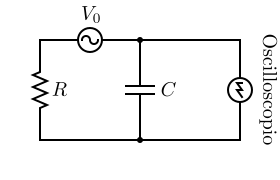
\includegraphics[width=\textwidth]{circuito_osc_C.pdf}
        \caption{Misure ai capi di C}
        \label{fig:circuito C}
    \end{subfigure}
    \caption{Schema circuito}
  \end{figure}

\section{Strumenti e materiali}

\begin{itemize}
    \item Generatore di tensione AC
    \item Multimetro digitale (utilizzato come ohmetro)
    \item Oscilloscopio
    \item Cavi
    \item Breadboard
    \item Resistore
    \item Condensatore
\end{itemize}

\section{Onda quadra} \label{sec:onda quadra}

La prima parte dell'esperimento consiste nell'applicare ai capi del circuito una tensione variabile secondo un'onda quadra di ampiezza \(V_{0}\). La frequenza dell'onda è stata scelta in modo da permettere al condensatore di completare il regime transitorio, passando da una tensione \(V_{0}/2\) fino ad una tensione \(- V_{0}/2\). La curva osservata nell'oscilloscopio rappresenta la tensione \(V_{C}\) ai capi del condensatore in funzione del tempo \(t\) e segue l'\autoref{eq:regime transitorio onda quadra}.

\begin{equation} \label{eq:regime transitorio onda quadra}
    V_{C} = V_{0} \cdot e^{-t/RC} - V_{0}/2
\end{equation}

Per prendere le misure il sistema di riferimento è stato traslato in modo da porre come zero delle ordinate il valore \(- V_{0}/2\) e ottenere l'\autoref{eq:regime transitorio condensatore}.

\begin{equation} \label{eq:regime transitorio condensatore}
    V = V_{0} \cdot e^{-t/RC}
\end{equation}

Noto il valore di \(R = (1.874 \pm 0.004) \; \unit{k\Omega}\) (misurato con il multimetro) si vuole ottenere il valore di \(C\).

\subsection{Dati ed errori}

Sull'oscilloscopio è stato fissato il primo cursore in corrispondenza dell'asintoto della curva a \(- V_{0}/2\); questo sarà lo zero delle ordinate. \\
Il secondo cursore è stato fatto variare in modo da ottenere la differenza di potenziale al variare del tempo. Le misure ottenute sono riportate, insieme ai loro errori già arrotondati, nella \autoref{tab:misure onda quadra}.

\begin{table}[ht!]
    \centering
    \caption{Misure dell'onda quadra}
    \import{../tables/}{onda_quadra_Vt.tex}
    \label{tab:misure onda quadra}
\end{table}

\subsection{Analisi dati}

\begin{equation*}
    V = V_{0} \cdot e^{-t/RC} \implies \ln(V) = \ln(V_{0} \cdot e^{-t/RC}) = \ln(V_{0}) - \frac{t}{RC}
\end{equation*}

Riportando le misure in un grafico semi-logaritmico (come in \autoref{fig:onda quadra pendenze}), ci si aspetta di ottenere una funzione lineare.

\begin{figure}[ht!]
    \includegraphics{onda_quadra_V(t)_pendenze.pdf}
    \caption{Grafico semi-logaritmico delle misure dell'onda quadra}
    \label{fig:onda quadra pendenze}
\end{figure}

La retta di massima pendenza passa per i punti \((-0.2, 7)\) e \((35, 0.6)\), mentre la retta di minima pendenza passa per i punti \((0.2, 7)\) e \((34, 0.5)\).

\begin{equation*}
    m_{max} = \frac{\ln(7/0.6)}{- 0.2 - 35} = - 0.06979
    \qquad
    m_{min} = \frac{\ln(7/0.5)}{0.2 - 34} = - 0.07808
\end{equation*}

\begin{align*}
    m_{best} &= \frac{m_{max} + m_{min}}{2} = - 0.0739 \approx - 0.074 \\
    \delta m &= \frac{m_{max} - m_{min}}{2} = 0.0041 \approx 0.004
\end{align*}

\begin{equation}
    m = - 0.074 \pm 0.004
\end{equation}

\newpage

Essendo \(m = - \dfrac{1}{RC}\) e conoscendo il valore di \(R = (1.874 \pm 0.004) \; \unit{k\Omega}\), calcoliamo $C$.

\begin{align*}
    \varepsilon_R &= \frac{0.004}{1.874} = 0.0021 \approx 0.002 \\
    \varepsilon_m &= \frac{0.004}{0.074} = 0.054 \approx 0.05 \\
    \varepsilon_C &= \sqrt{\varepsilon_R^{2} + \varepsilon_m^{2}} = 0.050
\end{align*}

\begin{equation}
    C =  -\frac{1}{m R} = 7.21 \pm 0.36 \approx (7.2 \pm 0.4) \; \unit{nF}
\end{equation}

\section{Onda sinusoidale}

La seconda parte dell'esperimento consiste nel sottoporre il circuito a un regime di tensione sinusoidale, variando la frequenza in entrata; abbiamo poi misurato la tensione in entrata e uscita del circuito ai capi di $C$ e ai capi di $R$, così come il suo tempo di risposta. Con questi dati abbiamo determinato il modulo della \emph{funzione di trasferimento} $|A|$, la sua fase $\varphi$ e la frequenza di taglio $f_{0}$.

Per indicare il componente in esame, nei nomi delle variabili è stato inserito a pedice $C$ per le misure del condensatore ed $R$ per quelle del resistore.

\subsection{Funzione di trasferimento ai capi di $C$}

\subsubsection{Dati ed errori}

Nella \autoref{tab:misure onda sinusoidale C} sono riportati i risultati delle misurazioni effettuate con i relativi errori

\begin{table}[ht!]
    \centering
    \caption{Misure dell'onda sinusoidale ai capi di $C$}
    \import{../tables/}{onda_sin_VC.tex}
    \label{tab:misure onda sinusoidale C}
\end{table}

\subsubsection{Analisi dati}

Con i dati raccolti si calcola il modulo della funzione di trasferimento $|A_{C}|$ al variare della frequenza utilizzando l'\autoref{eq:funzione di trasferimento C}

\begin{align} \label{eq:funzione di trasferimento C}
    \begin{split}
        |A_{C}| &= \frac{V_{out}}{V_{in}} \\
        \varepsilon_{|A_{C}|} &= \frac{\delta V_{out}}{V_{out}} + \frac{\delta V_{in}}{V_{in}}
    \end{split}
\end{align}

\begin{table}[ht!]
    \centering
    \caption{Valori di $|A_{C}|$}
    \import{../tables/}{onda_sin_AC.tex}
    \label{tab:funzione di trasferimento C}
\end{table}

Riportando le misure della \autoref{tab:funzione di trasferimento C} in un grafico logaritmico $|A_{C}|(f)$ si ottiene la \autoref{fig:funzione di trasferimento C}.

\begin{figure}[ht!]
    \includegraphics{onda_sin_AC(f).pdf}
    \caption{Grafico logaritmico di $|A_{C}|(f)$}
    \label{fig:funzione di trasferimento C}
\end{figure}

\newpage

Si osserva che il modulo della funzione di trasferimento, in scala logaritmica, assume un andamento lineare a frequenze elevate; è possibile quindi tracciare una retta di pendenza $-1$ passante per i punti situati all'estrema destra del grafico. Questa retta interseca l'asintoto orizzontale $|A_{C}| = 1$ alla frequenza di taglio $f_{C}$.

\begin{figure}[ht!]
    \includegraphics{onda_sin_AC(f)_taglio.pdf}
    \caption{Grafico della stima della frequenza di taglio}
    \label{fig:frequenza di taglio C}
\end{figure}

\begin{figure}[ht!]
    \includegraphics{onda_sin_AC(f)_taglio_frequenza.pdf}
    \caption{Zoom intersezione rette}
    \label{fig:frequenza di taglio C zoom}
\end{figure}

Abbiamo riportato uno zoom sull'intersezione delle rette in \autoref{fig:frequenza di taglio C zoom}.

\begin{align*}
    f_{C \; min} &= 12.0 \; kHz \\
    f_{C \; max} &= 12.5 \; kHz
\end{align*}

\begin{align*}
    f_{C \; best} &= \frac{f_{C \; max} + f_{C \; min}}{2} = 12.25 \approx 12.3 \; kHz \\
    \delta f_{C} &= \frac{f_{C \; max} - f_{C \; min}}{2} = 0.25 \approx 0.3 \; kHz
\end{align*}

Quindi il valore di \(f_{C} = (12.3 \pm 0.3) \; kHz\).

\rule{\textwidth}{1pt}

Con i dati della \autoref{tab:misure onda sinusoidale C}, calcoliamo la fase $\varphi_{C}(f)$ con l'\autoref{eq:fase C}; i risultati ottenuti sono nella \autoref{tab:fase di C}.

\begin{align} \label{eq:fase C}
    \begin{split}
        \varphi_{C} &= tf + 2k\pi \qquad k \in \mathbb{Z} \\
        \delta \varphi_{C} &= \frac{\delta t}{t} \varphi_{C}
    \end{split}
\end{align}

\begin{table}[ht!]
    \centering
    \caption{Valori di $\varphi_{C}$}
    \import{../tables/}{onda_sin_phiC.tex}
    \label{tab:fase di C}
\end{table}


\begin{figure}[ht!]
    \includegraphics{onda_sin_phi(f)_C.pdf}
    \caption{Grafico di $\varphi_{C}(f)$}
    \label{fig:fase C}
\end{figure}

\newpage

Successivamente sono state tracciate due rette passanti per i punti più vicini ad $f_{C}$ dove ci si aspetta un andamento lineare (\autoref{fig:rette fase C}).

\begin{figure}[ht!]
    \includegraphics{onda_sin_phi(f)_C_intercette.pdf}
    \caption{Rette intorno a $f_{C}$}
    \label{fig:rette fase C}
\end{figure}

\newpage

L'intersezione delle rette di massima e minima intercetta con $\varphi_{C} = -\pi/4$ è compatibile con il valore di $f_{C}$ calcolato precedentemente.

%%%%%%%%%%%%%%%%%%%%%%%%%%%%%%%%%% blocco opzionale
%Abbiamo quindi tracciato le rette di massima e minima intercetta passanti per i punti $(f_{0} - \delta f_{0}, -\pi/4)$ e $(f_{0} + \delta f_{0}, -\pi/4)$ in modo da poter osservare come il punto $(15.55, -0.90)$ è sufficientemente vicino alla frequenza di taglio da intersecare le rette con le sue barre d'errore.

% Per trovare la pendenza delle rette da tracciare, abbiamo valutato la derivata di (...)
%%%%%%%%%%%%%%%%%%%%%%%%%%%%%%%%%% blocco opzionale

\subsection{Funzione di trasferimento ai capi di $R$}

\subsubsection{Dati ed errori}

Nella \autoref{tab:misure onda sinusoidale R} sono riportati i risultati delle misurazioni effettuate con i relativi errori

\begin{table}[ht!]
    \centering
    \caption{Misure dell'onda sinusoidale ai capi di $R$}
    \import{../tables/}{onda_sin_VR.tex}
    \label{tab:misure onda sinusoidale R}
\end{table}


\subsubsection{Analisi dati}

Con i dati raccolti si calcola il modulo della funzione di trasferimento $|A_{R}|$ al variare della frequenza utilizzando l'\autoref{eq:funzione di trasferimento R}

\begin{align} \label{eq:funzione di trasferimento R}
    \begin{split}
        |A_{R}| &= \frac{V_{out}}{V_{in}} \\
        \varepsilon_{|A_{R}|} &= \frac{\delta V_{out}}{V_{out}} + \frac{\delta V_{in}}{V_{in}}
    \end{split}
\end{align}

\begin{table}[ht!]
    \centering
    \caption{Valori di $|A_{R}|$}
    \import{../tables/}{onda_sin_AR.tex}
    \label{tab:funzione di trasferimento R}
\end{table}

Riportando le misure della \autoref{tab:funzione di trasferimento R} in un grafico logaritmico $|A_{R}|(f)$ si ottiene la \autoref{fig:funzione di trasferimento R}

\begin{figure}[ht!]
    \includegraphics{onda_sin_AR(f).pdf}
    \caption{Grafico logaritmico di $|A_{R}|(f)$}
    \label{fig:funzione di trasferimento R}
\end{figure}

\newpage

Nella funzione $|A_{R}|$ si avrà un andamento lineare a basse frequenze; tracciamo in questo caso una retta di pendenza $1$ passante per i punti situati all'estrema sinistra del grafico. Questa retta interseca l'asintoto orizzontale $|A_{R}| = 1$ alla frequenza di taglio $f_{R}$.

\begin{figure}[ht!]
    \includegraphics{onda_sin_AR(f)_taglio.pdf}
    \caption{Grafico della stima della frequenza di taglio}
    \label{fig:frequenza di taglio R}
\end{figure}

\newpage

Abbiamo riportato uno zoom sull'intersezione delle rette in \autoref{fig:frequenza di taglio R zoom}.

\begin{figure}[ht!]
    \includegraphics{onda_sin_AR(f)_taglio_frequenza.pdf}
    \caption{Zoom intersezione rette}
    \label{fig:frequenza di taglio R zoom}
\end{figure}

\begin{align*}
    f_{R \; min} &= 12.2 \; kHz \\
    f_{R \; max} &= 12.8 \; kHz
\end{align*}

\begin{align*}
    f_{R \; best} &= \frac{f_{R \; max} + f_{R \; min}}{2} = 12.5  \; kHz \\
    \delta f_{R} &= \frac{f_{R \; max} - f_{R \; min}}{2} = 0.3 \; kHz
\end{align*}

Quindi il valore di \(f_{R} = (12.5 \pm 0.3) \; kHz\).

\rule{\textwidth}{1pt}

Con i dati della \autoref{tab:misure onda sinusoidale R}, calcoliamo la fase $\varphi_{R}(f)$ con l'\autoref{eq:fase R}; i risultati ottenuti sono nella \autoref{tab:fase di R}.

\begin{align} \label{eq:fase R}
    \begin{split}
        \varphi_{R} &= tf + 2k\pi \qquad k \in \mathbb{Z} \\
        \delta \varphi_{R} &= \frac{\delta t}{t} \varphi_{R}
    \end{split}
\end{align}

\begin{table}[ht!]
    \centering
    \caption{Valori di $\varphi_{R}$}
    \import{../tables/}{onda_sin_phiR.tex}
    \label{tab:fase di R}
\end{table}


\begin{figure}[ht!]
    \includegraphics{onda_sin_phi(f)_R.pdf}
    \caption{Grafico di $\varphi_{R}(f)$}
    \label{fig:fase R}
\end{figure}

\newpage

Successivamente sono state tracciate due rette passanti per i punti più vicini ad $f_{R}$ dove ci si aspetta un andamento lineare (\autoref{fig:rette fase R}).

\begin{figure}[ht!]
    \includegraphics{onda_sin_phi(f)_R_intercette.pdf}
    \caption{Rette intorno a $f_{R}$}
    \label{fig:rette fase R}
\end{figure}

\newpage

L'intersezione delle rette di massima e minima intercetta con $\varphi_{R} = \pi/4$ è compatibile con il valore di $f_{R}$ calcolato precedentemente.

\section{Conclusioni}

I valori di $f_{C}$ ed $f_{R}$ ricavati:

\begin{align*}
    f_{C} &= (12.3 \pm 0.3) \; kHz \\
    f_{R} &= (12.5 \pm 0.3) \; kHz
\end{align*}

\begin{figure}[ht!]
    \includegraphics{f_0_compatibili.pdf}
    \caption{Compatibilità di $f_{C}$ ed $f_{R}$}
    \label{fig:fC ed fR compatibili}
\end{figure}

risultano compatibili, come è possibile vedere nella \autoref{fig:fC ed fR compatibili}. Possiamo dare un valore finale di $f_{0} = (12.4 \pm 0.2) \; kHz$.

Con questo valore appena ottenuto, calcoliamo $\omega_{0} = 2 \pi f_{0} = 77.91 \pm 1.26 \approx (77.9 \pm 1.3) \; rad/ms$.

Il tempo caratteristico del circuito si può calcolare sia a partire da $\omega_{0}$

\begin{equation*}
    \tau_{1} = \frac{1}{\omega_{0}} = 12.84 \pm 0.21 \approx (12.8 \pm 0.2) \; \mu s
\end{equation*}

sia dalle misure di $R$ e $C$ trovate nella \autoref{sec:onda quadra}.

\begin{align*}
    R &= (1.874 \pm 0.004) \; \unit{k\Omega} \\
    C &= (7.2 \pm 0.4) \; \unit{nF}
\end{align*}

\begin{equation*}
    \tau_{2} = RC = 13.51 \pm 0.73 \approx (13.5 \pm 0.7) \; \mu s
\end{equation*}

\begin{figure}[ht!]
    \includegraphics{tau_compatibili.pdf}
    \caption{Compatibilità di $\tau_{1}$ e $\tau_{2}$}
    \label{fig:tau compatibili}
\end{figure}
 
Si verifica che i due $\tau_{1,2}$ sono compatibili, con un valore finale di $\tau = (12.90 \pm 0.10) \mu s$.

% \appendix
% \section{Frequenza dell'onda quadra}
% todo

\end{document}
